\documentclass[9pt,aspectratio=169]{beamer}

\usetheme{graham}

\title{Probability}
\subtitle[Graham Middle School]{Graham Middle School Math Olympiad Team}

\begin{document}

\maketitle

\begin{frame}{Probability}
  \begin{columns}[T]
    \begin{column}{0.5\textwidth}
      \begin{definition}
        An \textbf{outcome} is a possible result of an experiment.
      \end{definition}

      \begin{wrapfigure}[7]{r}{0.25\textwidth}%
        \vspace{-1em}
        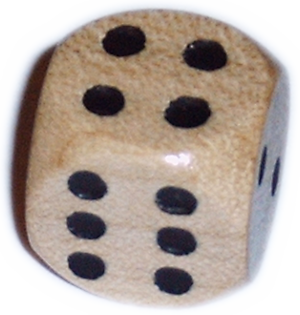
\includegraphics[width=0.3\textwidth]{03 - Probability/dice-4.png}
      \end{wrapfigure}
      We say "the outcome of throwing the dice was $4$." The experiment was throwing the die and its result (outcome) was that the face with $4$ pips on it came up.\medskip
  
      Probability problems are either based on \emph{countable} outcomes or on outcomes that are not countable. The later case is called \emph{geometric probability} or \emph{continuous probability}.

      \begin{definition}
        If the number of outcomes is countable and \emph{if all oucomes have the same probability}, then \mbox{the~\textbf{probability}} of desired oucome is:
        \[ P = \frac{\text{(number of desired outcomes)}}{\text{(total number of events)}}. \]
        \vspace*{-1ex}
      \end{definition}
    \end{column}
    \begin{column}{0.5\textwidth}
      \begin{problem}
        {\color{textBlue} Example:} We write each of the names of all $30$ students in a math club on a card and we draw a card at random. If there are $14$ sixth-graders, $9$ seventh-graders, and $7$ eighth-graders in this club, what is the probability of the name on the card being that of a sixth-grader? 
      \end{problem}
      The total number of \emph{outcomes} is all students in the club. The desired \emph{outcomes} are all sixth-graders. So \emph{probability} is
      \[
        P = \frac{14}{30} = \frac{7}{15}.
      \]

      \begin{definition}
        In the \emph{geometric case}, the \textbf{probability} of a desired outcome is calculated as the ratio:
        \[ P = \frac{\text{(desired area)}}{\text{(total area)}}. \]
        \vspace*{-1.5ex}
      \end{definition}

      Probabilities in any case are always between $0$ and $1$, inclusive.
    \end{column}
  \end{columns}
\end{frame}

\begin{frame}{Addition rule for probability}
  \begin{columns}[T]
    \begin{column}{0.5\textwidth}
      \begin{problem}
        What is the probability of choosing \emph{an ace} \textbf{or} \emph{a king} from a full deck of $52$ cards?
      \end{problem}
      \begin{wrapfigure}[6]{r}{0.20\textwidth}%
        \vspace{-1em}
        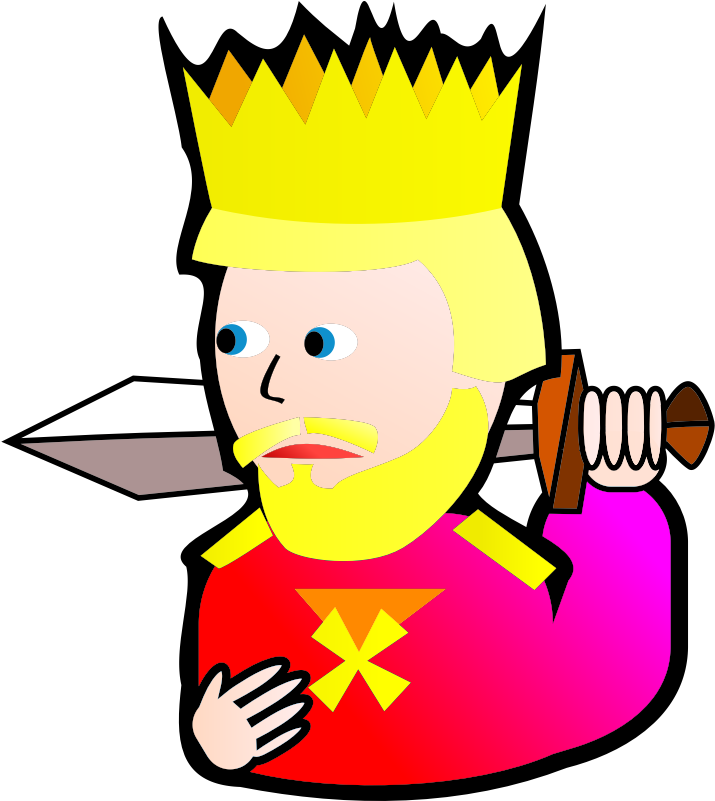
\includegraphics[width=0.25\textwidth]{03 - Probability/king-clip-art.png}
      \end{wrapfigure}
      \mbox{A card that we got from the deck of cards} may not be both an ace and a king. So we have $4$ \emph{oucomes} of getting an ace and $4$ \emph{oucomes} of getting a king. The result number of \emph{desired oucomes} is $8$. The \emph{total number of possible outcomes} is $52$.
      The total probability is
      \[ P = \frac{4 + 4}{52} = \frac{8}{52} = \frac{2}{13}. \]
      We also may count the probability in other way. The \emph{probability} of getting an ace is $4/52$ and the \emph{probability} of getting a king is also $4/52$. Since both cases are good for us, the total probability is
      \[ P = \frac{4}{52} + \frac{4}{52} = \frac{1}{13} + \frac{1}{13} = \frac{2}{13}. \]
    \end{column}
    \begin{column}{0.5\textwidth}
      \begin{definition}
        If two events are \emph{oucomes} of one experiment and they \emph{may not happen together}, then \emph{probability} of any of this event is \textbf{sum of their probabilities}
        \[ P(A\ \text{or}\ B) = P(A) + P(B). \]
        \vspace*{-2.5ex}          
      \end{definition}

      \begin{problem}
        What is the probability of choosing \emph{a multiple of $4$} or \emph{a multiple of $5$} from a numbers from $1$ to $100$?
      \end{problem}
      The probability of getting a multiple of $4$ is $25/100$, the probability of getting a multiple of $5$ is $20/100$. But there are multiples of $20$, which we counted twice. To make up for this case, we need to subtract the probability of getting a multiple of $20$, which is $5/100$. So total probability would be
      \[
        P = \frac{25}{100} + \frac{20}{100} - \frac{5}{100} = \frac{25 + 20 - 5}{100} = \frac{40}{100} = \frac{2}{5}.
      \]
      \begin{definition}
        So the \emph{probability of two events} of one experiment
        \[ P(A\ \text{or}\ B) = P(A) + P(B) - P(A\ \text{and}\ B). \]
        \vspace*{-2.5ex}          
      \end{definition}
    \end{column}
  \end{columns}
\end{frame}

\begin{frame}{Multiplication rule for probability}
  \begin{columns}[T]
    \begin{column}{0.5\textwidth}
      \begin{problem}
        If the experiment \emph{"throw a die and toss a coin"} is performed, what is the probability of the event \emph{"a~$4$~and a tails"} to happen?
      \end{problem}
      \begin{wrapfigure}[4]{l}{0.2\textwidth}%
        \vspace{-1.6em}
        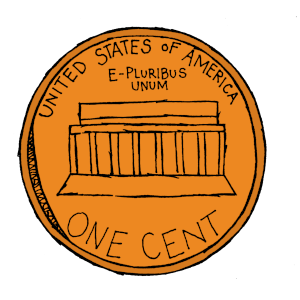
\includegraphics[width=0.23\textwidth]{03 - Probability/tail.png}
      \end{wrapfigure}
      Let's first throw a die. If $4$ didn’t happen, we don’t need to toss a coin, the desired event will not happen in any case. So we need to toss a~coin only when the die rolls~$4$. The $4$ has a probability of $1/6$ and, in this case only, we toss a coin and with a~probability of $1/2$ we will get tails. So the overall probability would be
      \[ P = \frac{1}{6} \cdot \frac{1}{2} = \frac{1}{12}. \] 

      \begin{definition}
        If two events are \emph{independent} the \textbf{probability} of both of them happen is \emph{a multiple of their probabilities}
        \[ P (A\ \text{and}\ B) = P (A) \cdot P (B). \] 
        \vspace*{-2ex} 
      \end{definition}
    \end{column}
    \begin{column}{0.5\textwidth}
      \begin{definition}
        The \textbf{conditional probability} of an event $E$ that depends on another event $F$ to happen is denoted 
        \[ P(E \mid F) \]
        and is probability of $E$ to happen if we know that $F$ has already happened.
      \end{definition}
      {\small We used that rule to solve the problem \emph{"throw a die and toss a coin"}.}
      \begin{definition}
        If two events are \emph{dependent} the \textbf{probability} of both of them happen is
        \[ P (A\ \text{and}\ B) = P (A) \cdot P (B \mid A). \] 
        \vspace*{-2.5ex} 
      \end{definition}
      {\small
        \begin{problem}
          What is the probability of choosing \emph{an ace} \textbf{and then} \emph{a~king} from a full deck of $52$ cards?
        \end{problem}
        The probability to choose an ace is $4/52$. Then we selecting a king from the deck without one card, so the probability to choose a king is $4/51$. The total probability~is
        \[ P(A \text{ and then } K) = P(A) \cdot P(K \mid A) = \frac{4}{52} \cdot \frac{4}{51} = \frac{4}{663}. \]
      }
    \end{column}
  \end{columns}
\end{frame}

\begin{frame}{Using the negative case}
  \begin{columns}[T]
    \begin{column}{0.5\textwidth}
      All probable outcomes of one experiment is equal to all experiment. That mean that probability of all outcomes is 
      \[ P(\text{All outcomes}) = 1. \]
      \vspace*{-1em}
      \begin{problem}
        What is the probability if throwing the dice and not to get $4$. 
      \end{problem}
      There are $5$ outcomes that is desired: $1$, $2$, $3$, $5$, and $6$. So total probability would be 
      \[ P(\text{not throwing $4$}) = 5 \cdot \frac{1}{6} = \frac{5}{6}. \]
      From other hand there is only one event that is not desired, so we can calculate the same probability as
      \begin{multline*} 
        P(\text{not throwing $4$}) = \\
        = P(\text{all possible results}) - P(\text{throwing $4$}) = \\
        = 1 - \frac{1}{6} = \frac{5}{6}.
      \end{multline*}
    \end{column}
    \begin{column}{0.5\textwidth}
      \begin{definition}
        The \textbf{complement event} of a \emph{desired event $E$}, denoted as $\overline{E}$, is the event that $E$ does not occur. Since for any event we know whether it is desired or not
        \[ P(\overline{E}) = 1 - P(E). \]
        \vspace*{-2.5ex} 
      \end{definition}
      Sometimes that simplifies the solution.
      \begin{problem}
        We are draw $4$ cards from a full deck of cards. What is the probability to get \emph{at least one ace}?
      \end{problem}
      If we try to solve the problem using the \emph{conditional probability} we find out that number of cases is pretty big. But we may count the probability to \emph{not get any ace}.
      \[ P (\text{no ace}) = \frac{48}{52} \cdot \frac{47}{51} \cdot \frac{46}{50} \cdot \frac{45}{49} = \frac{38916}{54145} \approx 72\%.\]\\[-1ex]
      And probability to get \emph{an ace with $4$ cards} is
      \[ P (\text{at least one ace}) = 1 - \frac{38916}{54145} = \frac{15229}{54145} \approx 28 \%. \]
    \end{column}
  \end{columns}
\end{frame}

\begin{frame}{The birthday problem}
  \begin{columns}[T]
    \begin{column}{0.5\textwidth}
      \begin{problem}
        How many people need to attend a party until there is a $50\%$ chance that at least two guests share a birthday?
      \end{problem}
      It is easier to calculate the probability that \emph{no two people share a birthday}. 
      
      Les's start with the first guest. He don't share a birthday with anyone. So the probability is $1$.
      
      The second guest may share a birthday with the first guest with probability $364/365$. 
      
      The third one don't share a birthday with previous guests with probability $363/365$ and so on. 
      
      For $n$ guests
      \begin{multline*}
        P(\text{no shared birthday}) = \\
        = \frac{365}{365} \cdot \frac{364}{365} \cdot \frac{363}{365} \cdot \ldots \frac{365 - n + 1}{365} = \\ = \frac{365!}{(365-n)!} \cdot \frac{1}{365^n}.
      \end{multline*}
    \end{column}
    \begin{column}{0.5\textwidth}
      Using formula 
      \begin{multline*}
         P(\text{there is a shared birthday}) = \\ 
         = 1 - P(\text{no shared birthday})
      \end{multline*}
      we can calculate, using computer, the probability for any number of guests
      \begin{center}
        \vspace*{-1ex}   
        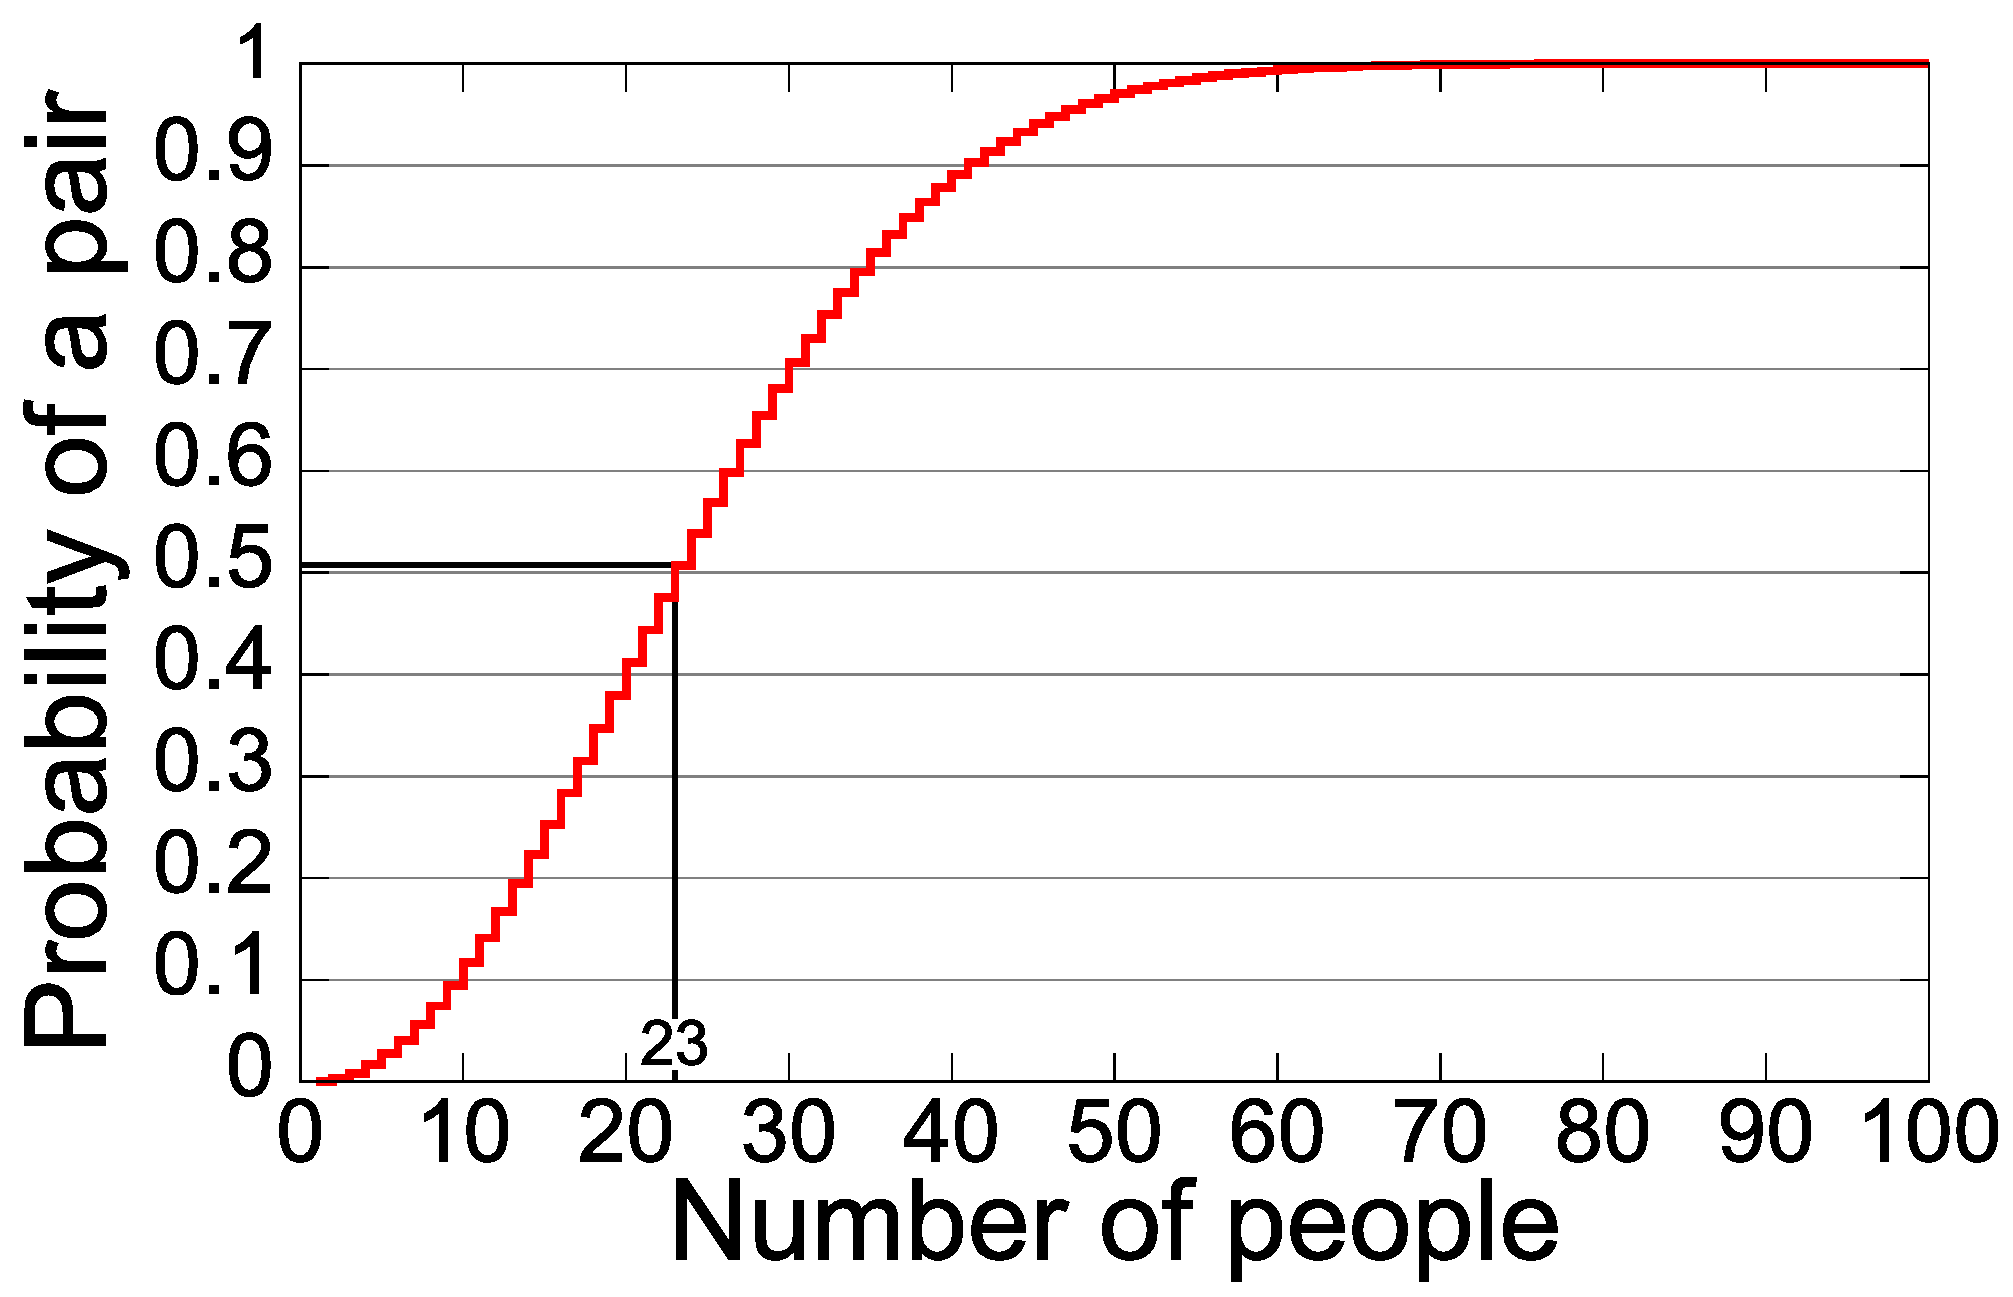
\includegraphics[width = 0.80\textwidth]{03 - Probability/Birthday_Paradox.pdf}
        \vspace*{-1ex}   
      \end{center} 
      So we may see that group of $23$ people has probability of $50.7\%$ to have a shared birthday, and group of $70$ people has probability of $99.9\%$ to~share a birthday.
    \end{column}
  \end{columns}
\end{frame}

% \begin{frame}{Title}
%   \begin{columns}[T]
%     \begin{column}{0.5\textwidth}
%     \end{column}
%     \begin{column}{0.5\textwidth}
%     \end{column}
%   \end{columns}
% \end{frame}
\end{document}
